% !TEX encoding = UTF-8 Unicode
\documentclass{beamer}
\usepackage{color}
\usepackage{url}
\usepackage[T2A]{fontenc}
\usepackage[utf8]{inputenc}
\usepackage{graphicx}
\usepackage{scrextend}
\usepackage[english,serbianc]{babel}
\usetheme{Copenhagen}
\usecolortheme{beaver}
\makeatother
\institute{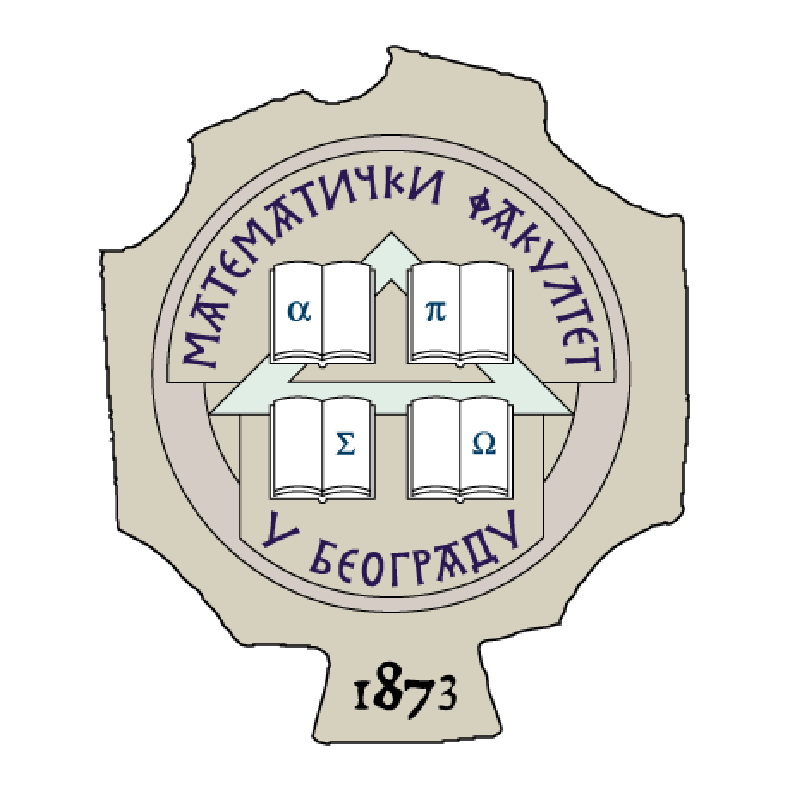
\includegraphics[scale=0.175]{matf-logo.eps}}
\setbeamertemplate{footline}
{
  \leavevmode%
  \hbox{%
  \begin{beamercolorbox}[wd=1.0\paperwidth,ht=2.25ex,dp=1ex,center]{title in head/foot}%
    \usebeamerfont{title in head/foot}\insertshorttitle\hspace*{3em}
    \insertframenumber{} / \inserttotalframenumber\hspace*{1ex}
  \end{beamercolorbox}}%
  \vskip0pt%
}
\makeatletter
\setbeamertemplate{navigation symbols}{}

\date{\tiny{24. новембар 2019.}}

\title{\textbf{Самсон Абрамски}}
\author{\small{Александра Лабовић, Игор Пајић,\\Александар Урошевић, Вељко Продан}}

\begin{document}
\frame{\titlepage}

% SLAJD
\begin{frame}
Номинација Самсона Абрамског за Краљевско друштво гласи:\\
\begin{addmargin}{2em}
\emph{„Самсон Абрамски се истиче за исконски допринос математичким темељима рачунања. Његово неприкосновено достигнуће је развој семантике игара као и теорија о рачунским процесима. Ово је довело до моћних апликација у проучавању програмских језика, нудећи нове одлучне увиде у природу секвенцијалности, стања, контроле, и многих других рачунарских карактеристика. То сада води новом развоју рачунарских програмских анализа и верификација. Једна важна нит, која такође важи као допринос у логици, је генерализација Жирарове Геометрије интеракција. Пре тога, Абрамски је направио важне доприносе апстракној интерпретацији, теорије домена, ламбда ($\lambda$) рачуну и паралелности. Он наставља да осветљава широк распон тема својим креативним и оштрим увидима, радећи нешто ново, и донесећи ред и јединство постојећем раду.”}
\end{addmargin}
\end{frame}

% SLAJD 
\begin{frame}
\frametitle{Увод}
\textbf{Самсон Абрамски} (рођен 12. марта 1953.) је информатичар са професуром Кристифора Странчеја на институту информатике Универзитета у Оксфорду. Допринео је областима теорије домена, ламбда рачунa, анализи строгости функција, теорија паралелности, категорије интеракција, геометрије интеракције, семантика игара и квантних рачунара.
\begin{center}
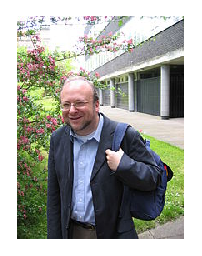
\includegraphics[scale=1.0]{lepisemi.eps}
\end{center}
\end{frame}

% SLAJD
\begin{frame}
\frametitle{Образовање}
Абрамски је образован у Хасмонејској гимназији за дечаке у Хендону, на Краљевском факултету у Кембриџу (дипломирао је као информатичар 1975. године, 1979. завршава магистар филозофије) и у Лондонском универзитету краљице Марије (докторат информатике 1988. са ментором Ричарда Борната)
\end{frame}

% SLAJD
\begin{frame}
\frametitle{Каријера и истраживања}

Радио је на следећим положајима:

\begin{itemize}
\item     програмер, корпорација ГЕЦ рачунари, 1976-1978
\item     предавач, Одсек за рачунарске науке и статистику, Лондонски универзитет краљице Марије, 1980-1983
\item     предавач, 1983-1988, читач, 1988-1990, професор, 1990-1995, Одсек за рачунарство, Империјални колеџ у Лондону
\item     професор теорије рачунарских наука, Универзитет у Единбургу, 1996-2000
\end{itemize}
\end{frame}

% SLAJD
\begin{frame}
\frametitle{Одабране публикације}
Самсон Абрамски је заједно са Давом Габеијем и Т.С.Е. Мејбаумом уредник шест томова Приручника логике у рачунарској науци. 
\begin{itemize}
\item     1992. Том 1: Позадина: Математичке структуре.
\item     1992. Том 2: Позадина: Рачунарске структуре.
\item     1995. Том 3: Семантичке структуре.
\item     1995. Том 4: Семантичко моделовање.
\item     2001. Том 5: Логичке и алгебарске методе.
\item 	  Том 6: Логичке методе у рачунарској науци.
\end{itemize}
\end{frame}

% SLAJD
\begin{frame}
\frametitle{Награде и почасти}
Абрамски је члан Краљевског друштва (2004.), члан Краљевског друштва Единбурга (2000.) и члан Европске академије (1993.). Такође је члан Уредништва Северно холандских студија логике и основа математике, и расправа о теоријској информатици Кембриџа. 
\end{frame}


% SLAJD
\begin{frame}
\frametitle{Одабране публикације}
Самсон Абрамски је објавио преко двеста публикација.

Неки од новијих радова Самсона Абрамског укључују: 

\begin{itemize}

\item    2013. Задовољење робустног ограничења и локалне скривене променљиве вредности у квантној механици. (са Г. Готлобом и П. Колеитисом). IJCAI 2013
\item    2012. Логичке неједнакости звона. (са Луцијеном Хардијем). У Физички преглед-{ Physical Review}- A. том 85. бр. АРТН 062114
\item    2010. Увод у категорије и категоричку логику. (са Н. Твевелексом). У Нове структуре за физику. -{New Structures for Physics}- Спрингер.

\end{itemize}
\end{frame}

% SLAJD
\begin{frame}
\frametitle{}
\begin{center}
Хвала на пажњи!
\end{center}
\begin{center}
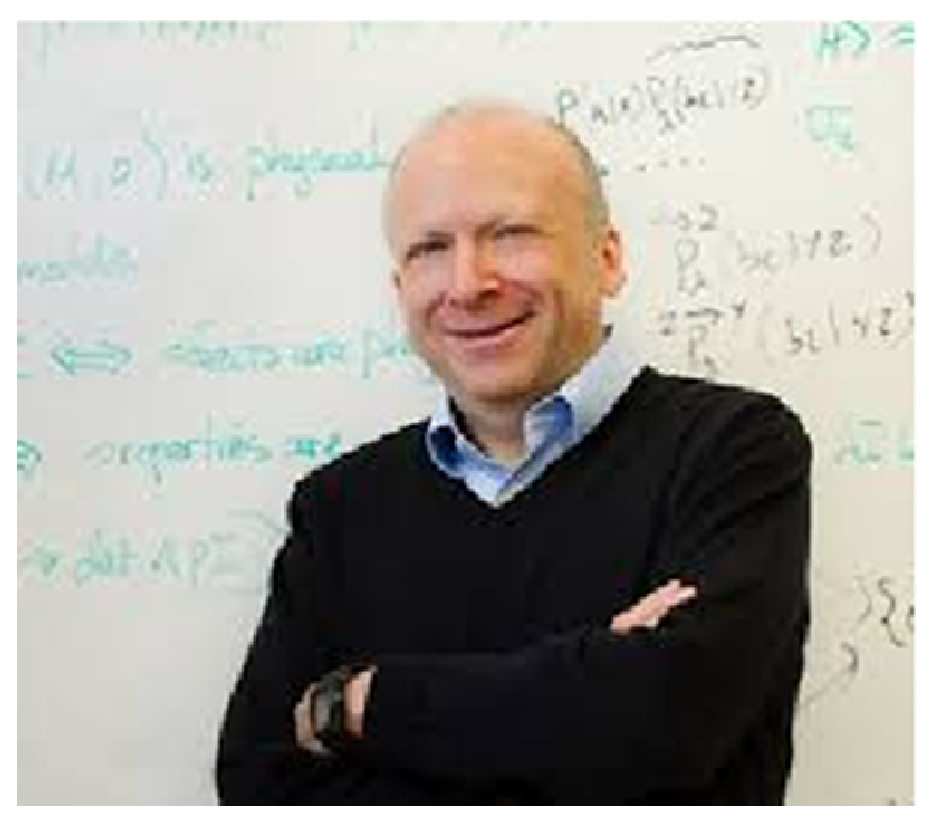
\includegraphics[scale=0.5]{index.eps}
\end{center}
\end{frame}


\end{document}
